\documentclass[a4paper,12pt]{book}
\usepackage[utf8]{inputenc}
\title{}
\author{Rachel Morris}
\date{\today}

\usepackage{rachwidgets}
\usepackage{fancyhdr}
\usepackage{lastpage}
\usepackage{dirtree}
\usepackage{boxedminipage}
\usepackage{colortbl} % cell bg colors

\setcounter{chapter}{4}
\setcounter{section}{1}
\newcommand{\laChapter}{4.2 The Composition Operation\ }
\newcounter{question}

\newcommand{\laClass}{CS 210\ }
\newcommand{\laSemester}{Fall 2017\ }

\pagestyle{fancy}
\fancyhf{}
\lhead{\laClass \laSemester}
\chead{}
\rhead{Ch \laChapter}
\rfoot{\thepage\ of \pageref{LastPage}}
\lfoot{\scriptsize Compiled by Rachel Morris, last updated \today}

\renewcommand{\headrulewidth}{2pt}
\renewcommand{\footrulewidth}{1pt}

\begin{document}

    %\toggletrue{answerkey}
    \togglefalse{answerkey}

    %------------------------------------------------------------------%
    %- Exercise Begin -------------------------------------------------%
    %------------------------------------------------------------------%

    \section{The Composition Operation}

    \subsection{Finding $f \circ g$, given $f$ and $g$}

    \notonkey{
        \begin{introNOHEAD}{}
            If $f : A \to B$ and $g : B \to C$, then we can build a new
            function called $(f \circ g)(x)$ that has the domain $A$
            and the codomain $C$, and that follows the rule
            $(f \circ g)(x) = f(g(x))$. We read $f \circ g$ as
            ``$f$ of $g$", or the composition of $f$ with $g$.

            To find $f \circ g$, you plug $f(x)$ into $g(x)$ and simplify.

            \paragraph{Example:} $f(x) = 2x + 1$ and $g(x) = x^{2} - 1$.
            What is $(f \circ g)(x)$? ~\\

            \begin{tabular}{l l}
                1. Plug $f(x)$ into $g(x)$: &
                $f(g(x))$
                \\ & $= f( x^{2} - 1 )$
                \\ & $= 2(x^{2} - 1) + 1$
                \\ \\
                2. Simplify: &
                $= 2x^{2} - 2x + 1$
                \\
                & $= 2x^{2} - 1$
            \end{tabular}
        \end{introNOHEAD}
    }{}
    
    % - QUESTION --------------------------------------------------%
    \stepcounter{question}
    \begin{questionNOGRADE}{\thequestion}

        Solve the following:

        \begin{itemize}
            \item[a.]   $f(x) = 2x-1$ and $g(x) = 3x$, what is $(f \circ g)(x)$?
                \solution{ ~\\ 
                    $f(g(x)) = f(3x) = 2(3x) - 1 = 6x - 1$
                }{ \vspace{1.5cm} }

            \item[b.]   $f(x) = 2x-1$ and $g(x) = 3x$, what is $(g \circ f)(x)$?
                \solution{ ~\\ 
                    $g(f(x)) = g(2x-1) = 3(2x-1) = 6x - 3$
                }{ \vspace{1.5cm} }

            \item[c.]   $f(x) = x^{2}$ and $g(x) = x+1$, what is $(f \circ g)(x)$?
                \solution{ ~\\ 
                    $f(g(x)) = f(x+1) = (x+1)^{2} = x^{2} + 2x + 1$
                }{ \vspace{1.5cm} }
            
            \item[d.]   $f(x) = x^{2}$ and $g(x) = x+1$, what is $(g \circ f)(x)$?
                \solution{ ~\\ 
                    $g(f(x)) = g(x^{2}) = x^{2} + 1$
                }{ \vspace{1cm} }
        \end{itemize}
        
    \end{questionNOGRADE}

    \notonkey{ \newpage }{ \hrulefill }

    \subsection{Finding $g$ based on $f$ and $f \circ g$}

    \notonkey{
        \begin{introNOHEAD}{}
            If we have $f$ and $f \circ g$, but need to find the
            function $g$, we can do this with substitution...

            \paragraph{Example:}
            $f(x) = 2x+1$ and $(f \circ g)(x) = 2x^{2} - 1$. What is
            $g(x)$? ~\\
            
            \begin{tabular}{l l}
                1. Use $a$ to symbolize $g(x)$. &
                    $a = g(x)$.
                \\ \\
                2. Rewrite $f(g(x))$ &
                    $f(g(x)) = f(a)$
                \\ \\
                3. Find $f(a)$ via the $f(x)$ function. &
                    $f(a) = 2a+1$
                \\ \\
                4. Set $f(a) = 2a+1$ equal \\
                    to $f(g(x)) = 2x^{2} - 1$. &
                    $2a+1  = 2x^{2} - 1$
                \\ \\
                5. Solve for $a$ to find $g(x)$. &
                    $2a+1  = 2x^{2} - 1$
                \\ & $2a = 2x^{2} - 1 - 1$
                \\ & $2a = 2x^{2} - 2$
                \\ & $a = x^{2} - 1$
            \end{tabular}

            Therefore, $g(x) = x^{2} - 1$.
        \end{introNOHEAD}
    }{}

    
    % - QUESTION --------------------------------------------------%
    \stepcounter{question}
    \begin{questionNOGRADE}{\thequestion}

        Solve the following:
        
        \begin{itemize}
            \item[a.]   $f(x) = 2x-1$ and $(f \circ g)(x) = 6x-1$, what is $g(x)$?
                \solution{ ~\\ 
                    $2a-1 = 6x-1$ \tab $2a = 6x$ \tab $a = 3x$ \\
                    $g(x) = 3x$
                }{ \vspace{1.5cm} }

            \item[b.]   $f(x) = x^{2}$ and $(f \circ g)(x) = x^{2} + 2x + 1$, what is $g(x)$?
                \solution{ ~\\ 
                    $a^{2} = x^{2} + 2x + 1$ \tab $a^{2} = (x+1)^{2}$ \tab{}
                    $a = x+1$ \\
                    $g(x) = x + 1$
                }{ \vspace{1.5cm} }

            \item[c.]   $f(x) = 3x-2$ and $(f \circ g)(x) = 12x + 7$, what is $g(x)$?
                \solution{ ~\\ 
                    $3a-2 = 12x + 7$ \tab $3a = 12x + 7 + 2$ \tab
                    $3a = 12x + 9$ \tab $a = 4x + 3$ \\
                    $g(x) = 4x + 3$
                }{ \vspace{1.5cm} }
            
        \end{itemize}
        
    \end{questionNOGRADE}

    \notonkey{ \newpage }{ \hrulefill }

    \subsection{Finding $f$ based on $g$ and $f \circ g$}

    \notonkey{
        \begin{introNOHEAD}{}
            If we have $g$ and $f \circ g$, but need to find the function
            $f$, we can use substitution in another way...

            \paragraph{Example:}
            $g(x) = x^{2} - 1$ and $(f \circ g)(x) = 2x^{2} - 1$.
            What is $f(x)$?~\\
            
            \begin{tabular}{l l}
                1. Beginning with $f(g(x))$,    \\
                    Set $a$ to the LHS of $g(x)$.
                & $a = x^{2} - 1$.
                \\ \\
                2. Solve for $x$:
                & $x^{2} = a + 1$
                \\ & $x = \sqrt{a+1}$
                \\ \\
                3. Rewrite $f(g(x))$:
                & $f(g(x)) = f(x^{2} - 1)$
                \\ \\
                4. Plug in $x = \sqrt{a+1}$
                & $f(a) = 2(\sqrt{a+1})^{2} - 1$
                \\ \\
                5. Simplify:
                & $f(a) = 2(a+1) - 1$
                \\ & $f(a) =2a + 2 - 1$
                \\ & $f(a) = 2a + 1$
            \end{tabular}

            So, $f(x) = 2x+1$.
        \end{introNOHEAD}
    }{}

    % - QUESTION --------------------------------------------------%
    \stepcounter{question}
    \begin{questionNOGRADE}{\thequestion}

        Solve the following:
        
        \begin{itemize}
            \item[a.]   $g(x) = 3x$ and $(f \circ g)(x) = 6x-1$. What is $f(x)$?
                \solution{ ~\\
                $a = 3x$. Solve for $x$: \tab $x = \frac{1}{3}(a)$. \\
                $f(g(x)) = 6x-1$, plug in $x$: \tab $f(a) = 6( \frac{1}{3} a) - 1$ \\
                Simplify: $f(a) = 2a - 1$. \\
                So $f(x) = 2x-1$.
                }{ \vspace{1.5cm} }

            \item[b.]   $g(x) = x+1$ and $(f \circ g)(x) = x^{2} + 2x + 1$. What is $f(x)$?
                \solution{ ~\\
                $a = x+1$ \tab $x = a - 1$ \\
                $f(g(x)) = f(a);$ \tab $f(a) = (a-1)^{2} + 2(a-1) + 1$ \\
                $f(a) = a^{2} - 2a + 1 + 2a - 2 + 1$ \\
                $f(a) = a^{2}$ \\
                So $f(x) = x^{2}$.
                }{ \vspace{1.5cm} }

            \item[c.]   $g(x) = 2x-1$ and $(f \circ g)(x) = 6x-1$. What is $f(x)$?
                \solution{ ~\\
                    $a = 2x - 1$ \tab $x = \frac{a+1}{2}$ \\
                    $f(g(x)) = f(a);$ \tab $f(a) = 6(\frac{a+1}{2}) - 1$ \\
                    $f(a) = 3(a+1)-1$ \tab $f(a) = 3a + 3 - 1$ \tab $f(a) = 3a + 2$ \\
                    So $f(x) = 3x+2$.
                }{ \vspace{1.5cm} }
            
        \end{itemize}
        
    \end{questionNOGRADE}
    
    \notonkey{ \newpage }{ \hrulefill }
    
    \subsection{More arrow diagrams}

    \notonkey{
        \begin{introNOHEAD}{}
            We can also use arrow diagrams to visually represent
            functions and compositions of functions.

            \paragraph{Example:} ~\\
                %\footnotesize 
                $f(x)$: Domain $A$ = \{1, 2\}, Codomain $B$ = \{3, 4\}, \\ \tab Rule \{ (1,3), (1,4), (2,4) \}, \\
                $g(x)$: Domain $B$ = \{3, 4\}, Codomain $D$ = \{f, g\}, \\ \tab Rule \{ (3,f), (4,g) \}. \\
                ~\\ Draw the diagrams for $f(x)$, $g(x)$, and $f(g(x))$.
                %\normalsize 

            \begin{center}
                \begin{tikzpicture}[arrow/.style = {thick,-stealth}]
                    \draw[fill=white] (0,0) rectangle (2,3);
                    \draw[fill=white] (3,0) rectangle (5,3);
                    \node [below] at (2.5,-0.5) {$f : A \to B$};
                    \filldraw (1, 1) circle (1pt) node[left]  { 1 };
                    \filldraw (1, 2) circle (1pt) node[left]  { 2 };
                    \filldraw (4, 1) circle (1pt) node[right] { 3 };
                    \filldraw (4, 2) circle (1pt) node[right] { 4 };
                    \draw[arrow] (1,1) -- (3.5,1);
                    \draw[arrow] (1,1) -- (3.5,1.8);
                    \draw[arrow] (1,2) -- (3.5,2);
                    
                    \draw[fill=white] (7,0) rectangle (9,3);
                    \draw[fill=white] (10,0) rectangle (12,3);
                    \node [below] at (9.5,-0.5) {$g : B \to C$};
                    \filldraw (8, 1) circle (1pt)   node[left] { 3 };
                    \filldraw (8, 2) circle (1pt)   node[left] { 4 };
                    \filldraw (11, 1) circle (1pt) node[right] { f };
                    \filldraw (11, 2) circle (1pt) node[right] { g };
                    \draw[arrow] (8,1) -- (10.5,1);
                    \draw[arrow] (8,2) -- (10.5,2);
                    
                    \draw[fill=white] (3.5,-3) rectangle (5.5,-6);
                    \draw[fill=white] (6.5,-3) rectangle (8.5,-6);
                    \node [below] at (6,-6.5) {$f \circ g : A \to C$};
                    \filldraw (4.5, -5) circle (1pt) node[left]  { 1 };
                    \filldraw (4.5, -4) circle (1pt) node[left]  { 2 };
                    \filldraw (7.5, -5) circle (1pt) node[right] { f };
                    \filldraw (7.5, -4) circle (1pt) node[right] { g };
                    \draw[arrow] (4.5,-4) -- (7,-4);
                    \draw[arrow] (4.5,-5) -- (7,-4.2);
                    \draw[arrow] (4.5,-5) -- (7,-5);
                    
                \end{tikzpicture}
            \end{center}
        \end{introNOHEAD}
    }{}
    
    \notonkey{ \newpage }{ \hrulefill }

    % - QUESTION --------------------------------------------------%
    \stepcounter{question}
    \begin{questionNOGRADE}{\thequestion}

        Finish the following diagrams:

        \begin{itemize}
            \item[a.] ~\\
                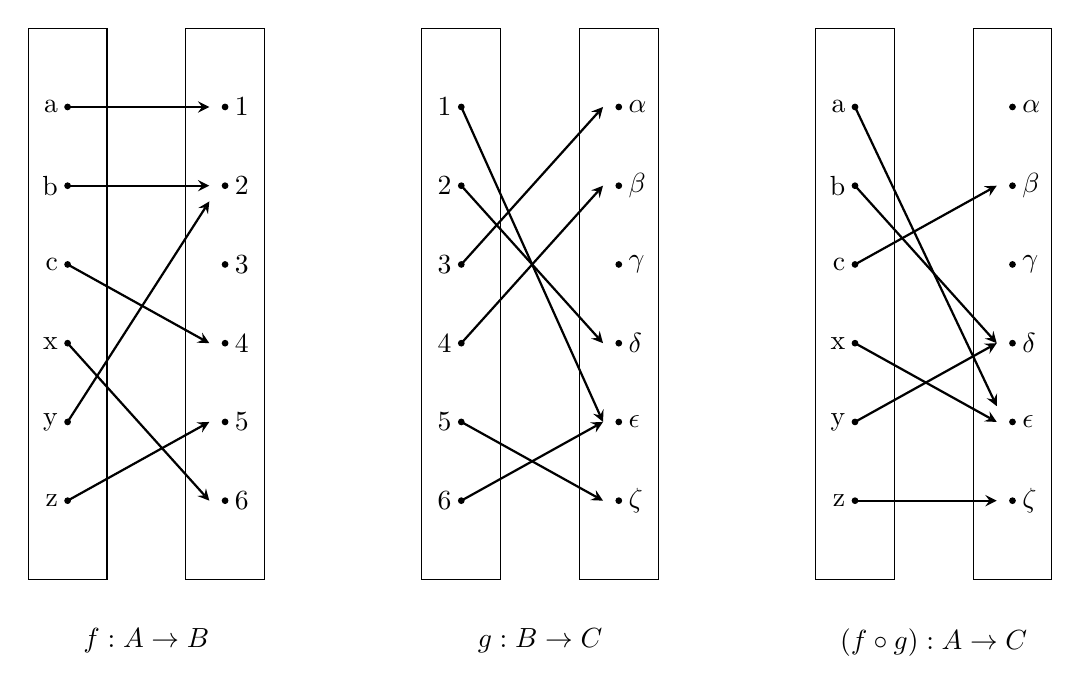
\begin{tikzpicture}[arrow/.style = {thick,-stealth}]
                    \node [below] at (1.5,-0.5) {$f : A \to B$};
                    \draw[fill=white] (0,0) rectangle (1,7);
                    \draw[fill=white] (2,0) rectangle (3,7);
                    \filldraw (0.5, 6) circle (1pt) node[left]  { a };
                    \filldraw (0.5, 5) circle (1pt) node[left]  { b };
                    \filldraw (0.5, 4) circle (1pt) node[left]  { c };
                    \filldraw (0.5, 3) circle (1pt) node[left]  { x };
                    \filldraw (0.5, 2) circle (1pt) node[left]  { y };
                    \filldraw (0.5, 1) circle (1pt) node[left]  { z };
                    
                    \filldraw (2.5, 6) circle (1pt) node[right]  { 1 };
                    \filldraw (2.5, 5) circle (1pt) node[right]  { 2 };
                    \filldraw (2.5, 4) circle (1pt) node[right]  { 3 };
                    \filldraw (2.5, 3) circle (1pt) node[right]  { 4 };
                    \filldraw (2.5, 2) circle (1pt) node[right]  { 5 };
                    \filldraw (2.5, 1) circle (1pt) node[right]  { 6 };
                    \draw[arrow] (0.5,6) -- (2.3,6);
                    \draw[arrow] (0.5,5) -- (2.3,5);
                    \draw[arrow] (0.5,4) -- (2.3,3);
                    \draw[arrow] (0.5,3) -- (2.3,1);
                    \draw[arrow] (0.5,2) -- (2.3,4.8);
                    \draw[arrow] (0.5,1) -- (2.3,2);

                    \node [below] at (6.5,-0.5) {$g : B \to C$};
                    \draw[fill=white] (5,0) rectangle (6,7);
                    \draw[fill=white] (7,0) rectangle (8,7);
                    \filldraw (5.5, 6) circle (1pt) node[left]  { 1 };
                    \filldraw (5.5, 5) circle (1pt) node[left]  { 2 };
                    \filldraw (5.5, 4) circle (1pt) node[left]  { 3 };
                    \filldraw (5.5, 3) circle (1pt) node[left]  { 4 };
                    \filldraw (5.5, 2) circle (1pt) node[left]  { 5 };
                    \filldraw (5.5, 1) circle (1pt) node[left]  { 6 };
                    
                    \filldraw (7.5, 6) circle (1pt) node[right]  { $\alpha$ };
                    \filldraw (7.5, 5) circle (1pt) node[right]  { $\beta$ };
                    \filldraw (7.5, 4) circle (1pt) node[right]  { $\gamma$ };
                    \filldraw (7.5, 3) circle (1pt) node[right]  { $\delta$ };
                    \filldraw (7.5, 2) circle (1pt) node[right]  { $\epsilon$ };
                    \filldraw (7.5, 1) circle (1pt) node[right]  { $\zeta$ };
                    \draw[arrow] (5.5,6) -- (7.3,2);
                    \draw[arrow] (5.5,5) -- (7.3,3);
                    \draw[arrow] (5.5,4) -- (7.3,6);
                    \draw[arrow] (5.5,3) -- (7.3,5);
                    \draw[arrow] (5.5,2) -- (7.3,1);
                    \draw[arrow] (5.5,1) -- (7.3,2);

                    \node [below] at (11.5,-0.5) {$(f \circ g) : A \to C$};
                    \draw[fill=white] (10,0) rectangle (11,7);
                    \draw[fill=white] (12,0) rectangle (13,7);
                    \filldraw (10.5, 6) circle (1pt) node[left]  { a };
                    \filldraw (10.5, 5) circle (1pt) node[left]  { b };
                    \filldraw (10.5, 4) circle (1pt) node[left]  { c };
                    \filldraw (10.5, 3) circle (1pt) node[left]  { x };
                    \filldraw (10.5, 2) circle (1pt) node[left]  { y };
                    \filldraw (10.5, 1) circle (1pt) node[left]  { z };
                    
                    \filldraw (12.5, 6) circle (1pt) node[right]  { $\alpha$ };
                    \filldraw (12.5, 5) circle (1pt) node[right]  { $\beta$ };
                    \filldraw (12.5, 4) circle (1pt) node[right]  { $\gamma$ };
                    \filldraw (12.5, 3) circle (1pt) node[right]  { $\delta$ };
                    \filldraw (12.5, 2) circle (1pt) node[right]  { $\epsilon$ };
                    \filldraw (12.5, 1) circle (1pt) node[right]  { $\zeta$ };

                    \solution{
                    \draw[arrow] (10.5,6) -- (12.3,2.2);
                    \draw[arrow] (10.5,5) -- (12.3,3);
                    \draw[arrow] (10.5,4) -- (12.3,5);
                    \draw[arrow] (10.5,3) -- (12.3,2);
                    \draw[arrow] (10.5,2) -- (12.3,3);
                    \draw[arrow] (10.5,1) -- (12.3,1);
                    }{}
                \end{tikzpicture}
            
            \item[b.] ~\\
                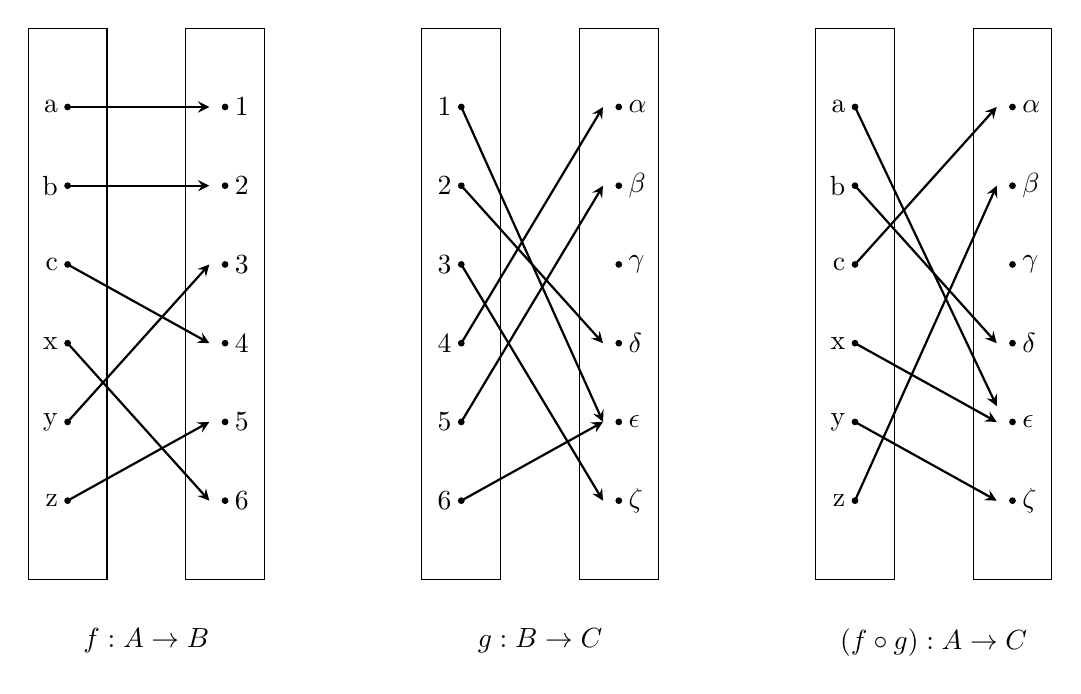
\begin{tikzpicture}[arrow/.style = {thick,-stealth}]
                    \node [below] at (1.5,-0.5) {$f : A \to B$};
                    \draw[fill=white] (0,0) rectangle (1,7);
                    \draw[fill=white] (2,0) rectangle (3,7);
                    \filldraw (0.5, 6) circle (1pt) node[left]  { a };
                    \filldraw (0.5, 5) circle (1pt) node[left]  { b };
                    \filldraw (0.5, 4) circle (1pt) node[left]  { c };
                    \filldraw (0.5, 3) circle (1pt) node[left]  { x };
                    \filldraw (0.5, 2) circle (1pt) node[left]  { y };
                    \filldraw (0.5, 1) circle (1pt) node[left]  { z };
                    \draw[arrow] (0.5,6) -- (2.3,6);
                    \draw[arrow] (0.5,5) -- (2.3,5);
                    \draw[arrow] (0.5,4) -- (2.3,3);
                    \draw[arrow] (0.5,3) -- (2.3,1);
                    \draw[arrow] (0.5,2) -- (2.3,4);
                    \draw[arrow] (0.5,1) -- (2.3,2);
                    
                    \filldraw (2.5, 6) circle (1pt) node[right]  { 1 };
                    \filldraw (2.5, 5) circle (1pt) node[right]  { 2 };
                    \filldraw (2.5, 4) circle (1pt) node[right]  { 3 };
                    \filldraw (2.5, 3) circle (1pt) node[right]  { 4 };
                    \filldraw (2.5, 2) circle (1pt) node[right]  { 5 };
                    \filldraw (2.5, 1) circle (1pt) node[right]  { 6 };

                    \node [below] at (6.5,-0.5) {$g : B \to C$};
                    \draw[fill=white] (5,0) rectangle (6,7);
                    \draw[fill=white] (7,0) rectangle (8,7);
                    \filldraw (5.5, 6) circle (1pt) node[left]  { 1 };
                    \filldraw (5.5, 5) circle (1pt) node[left]  { 2 };
                    \filldraw (5.5, 4) circle (1pt) node[left]  { 3 };
                    \filldraw (5.5, 3) circle (1pt) node[left]  { 4 };
                    \filldraw (5.5, 2) circle (1pt) node[left]  { 5 };
                    \filldraw (5.5, 1) circle (1pt) node[left]  { 6 };
                    
                    \filldraw (7.5, 6) circle (1pt) node[right]  { $\alpha$ };
                    \filldraw (7.5, 5) circle (1pt) node[right]  { $\beta$ };
                    \filldraw (7.5, 4) circle (1pt) node[right]  { $\gamma$ };
                    \filldraw (7.5, 3) circle (1pt) node[right]  { $\delta$ };
                    \filldraw (7.5, 2) circle (1pt) node[right]  { $\epsilon$ };
                    \filldraw (7.5, 1) circle (1pt) node[right]  { $\zeta$ };

                    \solution{
                    \draw[arrow] (5.5,6) -- (7.3,2);
                    \draw[arrow] (5.5,5) -- (7.3,3);
                    \draw[arrow] (5.5,4) -- (7.3,1);
                    \draw[arrow] (5.5,3) -- (7.3,6);
                    \draw[arrow] (5.5,2) -- (7.3,5);
                    \draw[arrow] (5.5,1) -- (7.3,2);
                    }{}

                    \node [below] at (11.5,-0.5) {$(f \circ g) : A \to C$};
                    \draw[fill=white] (10,0) rectangle (11,7);
                    \draw[fill=white] (12,0) rectangle (13,7);
                    \filldraw (10.5, 6) circle (1pt) node[left]  { a };
                    \filldraw (10.5, 5) circle (1pt) node[left]  { b };
                    \filldraw (10.5, 4) circle (1pt) node[left]  { c };
                    \filldraw (10.5, 3) circle (1pt) node[left]  { x };
                    \filldraw (10.5, 2) circle (1pt) node[left]  { y };
                    \filldraw (10.5, 1) circle (1pt) node[left]  { z };
                    
                    \filldraw (12.5, 6) circle (1pt) node[right]  { $\alpha$ };
                    \filldraw (12.5, 5) circle (1pt) node[right]  { $\beta$ };
                    \filldraw (12.5, 4) circle (1pt) node[right]  { $\gamma$ };
                    \filldraw (12.5, 3) circle (1pt) node[right]  { $\delta$ };
                    \filldraw (12.5, 2) circle (1pt) node[right]  { $\epsilon$ };
                    \filldraw (12.5, 1) circle (1pt) node[right]  { $\zeta$ };
                    \draw[arrow] (10.5,6) -- (12.3,2.2);
                    \draw[arrow] (10.5,5) -- (12.3,3);
                    \draw[arrow] (10.5,4) -- (12.3,6);
                    \draw[arrow] (10.5,3) -- (12.3,2);
                    \draw[arrow] (10.5,2) -- (12.3,1);
                    \draw[arrow] (10.5,1) -- (12.3,5);
                \end{tikzpicture}
            
        \end{itemize}
        
    \end{questionNOGRADE}
        
\end{document}








